%% bare_jrnl.tex
%% V1.4a
%% 2014/09/17
%% by Michael Shell
%% see http://www.michaelshell.org/
%% for current contact information.
%%
%% This is a skeleton file demonstrating the use of IEEEtran.cls
%% (requires IEEEtran.cls version 1.8a or later) with an IEEE
%% journal paper.
%%
%% Support sites:
%% http://www.michaelshell.org/tex/ieeetran/
%% http://www.ctan.org/tex-archive/macros/latex/contrib/IEEEtran/
%% and
%% http://www.ieee.org/

%%*************************************************************************
%% Legal Notice:
%% This code is offered as-is without any warranty either expressed or
%% implied; without even the implied warranty of MERCHANTABILITY or
%% FITNESS FOR A PARTICULAR PURPOSE! 
%% User assumes all risk.
%% In no event shall IEEE or any contributor to this code be liable for
%% any damages or losses, including, but not limited to, incidental,
%% consequential, or any other damages, resulting from the use or misuse
%% of any information contained here.
%%
%% All comments are the opinions of their respective authors and are not
%% necessarily endorsed by the IEEE.
%%
%% This work is distributed under the LaTeX Project Public License (LPPL)
%% ( http://www.latex-project.org/ ) version 1.3, and may be freely used,
%% distributed and modified. A copy of the LPPL, version 1.3, is included
%% in the base LaTeX documentation of all distributions of LaTeX released
%% 2003/12/01 or later.
%% Retain all contribution notices and credits.
%% ** Modified files should be clearly indicated as such, including  **
%% ** renaming them and changing author support contact information. **
%%
%% File list of work: IEEEtran.cls, IEEEtran_HOWTO.pdf, bare_adv.tex,
%%                    bare_conf.tex, bare_jrnl.tex, bare_conf_compsoc.tex,
%%                    bare_jrnl_compsoc.tex, bare_jrnl_transmag.tex
%%*************************************************************************


% *** Authors should verify (and, if needed, correct) their LaTeX system  ***
% *** with the testflow diagnostic prior to trusting their LaTeX platform ***
% *** with production work. IEEE's font choices and paper sizes can       ***
% *** trigger bugs that do not appear when using other class files.       ***                          ***
% The testflow support page is at:
% http://www.michaelshell.org/tex/testflow/



\documentclass[journal]{IEEEtran}
%
% If IEEEtran.cls has not been installed into the LaTeX system files,
% manually specify the path to it like:
% \documentclass[journal]{../sty/IEEEtran}





% Some very useful LaTeX packages include:
% (uncomment the ones you want to load)


% *** MISC UTILITY PACKAGES ***
%
%\usepackage{ifpdf}
% Heiko Oberdiek's ifpdf.sty is very useful if you need conditional
% compilation based on whether the output is pdf or dvi.
% usage:
% \ifpdf
%   % pdf code
% \else
%   % dvi code
% \fi
% The latest version of ifpdf.sty can be obtained from:
% http://www.ctan.org/tex-archive/macros/latex/contrib/oberdiek/
% Also, note that IEEEtran.cls V1.7 and later provides a builtin
% \ifCLASSINFOpdf conditional that works the same way.
% When switching from latex to pdflatex and vice-versa, the compiler may
% have to be run twice to clear warning/error messages.






% *** CITATION PACKAGES ***
%
%\usepackage{cite}
% cite.sty was written by Donald Arseneau
% V1.6 and later of IEEEtran pre-defines the format of the cite.sty package
% \cite{} output to follow that of IEEE. Loading the cite package will
% result in citation numbers being automatically sorted and properly
% "compressed/ranged". e.g., [1], [9], [2], [7], [5], [6] without using
% cite.sty will become [1], [2], [5]--[7], [9] using cite.sty. cite.sty's
% \cite will automatically add leading space, if needed. Use cite.sty's
% noadjust option (cite.sty V3.8 and later) if you want to turn this off
% such as if a citation ever needs to be enclosed in parenthesis.
% cite.sty is already installed on most LaTeX systems. Be sure and use
% version 5.0 (2009-03-20) and later if using hyperref.sty.
% The latest version can be obtained at:
% http://www.ctan.org/tex-archive/macros/latex/contrib/cite/
% The documentation is contained in the cite.sty file itself.
\usepackage{cite}
\usepackage{hyperref}
\usepackage{longtable}
\usepackage{color}


% *** GRAPHICS RELATED PACKAGES ***
%
\ifCLASSINFOpdf
   \usepackage[pdftex]{graphicx}
  % declare the path(s) where your graphic files are
  % \graphicspath{{../pdf/}{../jpeg/}}
  % and their extensions so you won't have to specify these with
  % every instance of \includegraphics
  % \DeclareGraphicsExtensions{.pdf,.jpeg,.png}
\else
  % or other class option (dvipsone, dvipdf, if not using dvips). graphicx
  % will default to the driver specified in the system graphics.cfg if no
  % driver is specified.
   \usepackage[dvips]{graphicx}
  % declare the path(s) where your graphic files are
  % \graphicspath{{../eps/}}
  % and their extensions so you won't have to specify these with
  % every instance of \includegraphics
  % \DeclareGraphicsExtensions{.eps}
\fi
% graphicx was written by David Carlisle and Sebastian Rahtz. It is
% required if you want graphics, photos, etc. graphicx.sty is already
% installed on most LaTeX systems. The latest version and documentation
% can be obtained at: 
% http://www.ctan.org/tex-archive/macros/latex/required/graphics/
% Another good source of documentation is "Using Imported Graphics in
% LaTeX2e" by Keith Reckdahl which can be found at:
% http://www.ctan.org/tex-archive/info/epslatex/
%
% latex, and pdflatex in dvi mode, support graphics in encapsulated
% postscript (.eps) format. pdflatex in pdf mode supports graphics
% in .pdf, .jpeg, .png and .mps (metapost) formats. Users should ensure
% that all non-photo figures use a vector format (.eps, .pdf, .mps) and
% not a bitmapped formats (.jpeg, .png). IEEE frowns on bitmapped formats
% which can result in "jaggedy"/blurry rendering of lines and letters as
% well as large increases in file sizes.
%
% You can find documentation about the pdfTeX application at:
% http://www.tug.org/applications/pdftex





% *** MATH PACKAGES ***
%
%\usepackage[cmex10]{amsmath}
% A popular package from the American Mathematical Society that provides
% many useful and powerful commands for dealing with mathematics. If using
% it, be sure to load this package with the cmex10 option to ensure that
% only type 1 fonts will utilized at all point sizes. Without this option,
% it is possible that some math symbols, particularly those within
% footnotes, will be rendered in bitmap form which will result in a
% document that can not be IEEE Xplore compliant!
%
% Also, note that the amsmath package sets \interdisplaylinepenalty to 10000
% thus preventing page breaks from occurring within multiline equations. Use:
%\interdisplaylinepenalty=2500
% after loading amsmath to restore such page breaks as IEEEtran.cls normally
% does. amsmath.sty is already installed on most LaTeX systems. The latest
% version and documentation can be obtained at:
% http://www.ctan.org/tex-archive/macros/latex/required/amslatex/math/





% *** SPECIALIZED LIST PACKAGES ***
%
%\usepackage{algorithmic}
% algorithmic.sty was written by Peter Williams and Rogerio Brito.
% This package provides an algorithmic environment for describing algorithms.
% You can use the algorithmic environment in-text or within a figure
% environment to provide for a floating algorithm. Do NOT use the algorithm
% floating environment provided by algorithm.sty (by the same authors) or
% algorithm2e.sty (by Christophe Fiorio) as IEEE does not use dedicated
% algorithm float types and packages that provide these will not provide
% correct IEEE style captions. The latest version and documentation of
% algorithmic.sty can be obtained at:
% http://www.ctan.org/tex-archive/macros/latex/contrib/algorithms/
% There is also a support site at:
% http://algorithms.berlios.de/index.html
% Also of interest may be the (relatively newer and more customizable)
% algorithmicx.sty package by Szasz Janos:
% http://www.ctan.org/tex-archive/macros/latex/contrib/algorithmicx/




% *** ALIGNMENT PACKAGES ***
%
%\usepackage{array}
% Frank Mittelbach's and David Carlisle's array.sty patches and improves
% the standard LaTeX2e array and tabular environments to provide better
% appearance and additional user controls. As the default LaTeX2e table
% generation code is lacking to the point of almost being broken with
% respect to the quality of the end results, all users are strongly
% advised to use an enhanced (at the very least that provided by array.sty)
% set of table tools. array.sty is already installed on most systems. The
% latest version and documentation can be obtained at:
% http://www.ctan.org/tex-archive/macros/latex/required/tools/


% IEEEtran contains the IEEEeqnarray family of commands that can be used to
% generate multiline equations as well as matrices, tables, etc., of high
% quality.




% *** SUBFIGURE PACKAGES ***
%\ifCLASSOPTIONcompsoc
%  \usepackage[caption=false,font=normalsize,labelfont=sf,textfont=sf]{subfig}
%\else
%  \usepackage[caption=false,font=footnotesize]{subfig}
%\fi
% subfig.sty, written by Steven Douglas Cochran, is the modern replacement
% for subfigure.sty, the latter of which is no longer maintained and is
% incompatible with some LaTeX packages including fixltx2e. However,
% subfig.sty requires and automatically loads Axel Sommerfeldt's caption.sty
% which will override IEEEtran.cls' handling of captions and this will result
% in non-IEEE style figure/table captions. To prevent this problem, be sure
% and invoke subfig.sty's "caption=false" package option (available since
% subfig.sty version 1.3, 2005/06/28) as this is will preserve IEEEtran.cls
% handling of captions.
% Note that the Computer Society format requires a larger sans serif font
% than the serif footnote size font used in traditional IEEE formatting
% and thus the need to invoke different subfig.sty package options depending
% on whether compsoc mode has been enabled.
%
% The latest version and documentation of subfig.sty can be obtained at:
% http://www.ctan.org/tex-archive/macros/latex/contrib/subfig/




% *** FLOAT PACKAGES ***
%
%\usepackage{fixltx2e}
% fixltx2e, the successor to the earlier fix2col.sty, was written by
% Frank Mittelbach and David Carlisle. This package corrects a few problems
% in the LaTeX2e kernel, the most notable of which is that in current
% LaTeX2e releases, the ordering of single and double column floats is not
% guaranteed to be preserved. Thus, an unpatched LaTeX2e can allow a
% single column figure to be placed prior to an earlier double column
% figure. The latest version and documentation can be found at:
% http://www.ctan.org/tex-archive/macros/latex/base/


%\usepackage{stfloats}
% stfloats.sty was written by Sigitas Tolusis. This package gives LaTeX2e
% the ability to do double column floats at the bottom of the page as well
% as the top. (e.g., "\begin{figure*}[!b]" is not normally possible in
% LaTeX2e). It also provides a command:
%\fnbelowfloat
% to enable the placement of footnotes below bottom floats (the standard
% LaTeX2e kernel puts them above bottom floats). This is an invasive package
% which rewrites many portions of the LaTeX2e float routines. It may not work
% with other packages that modify the LaTeX2e float routines. The latest
% version and documentation can be obtained at:
% http://www.ctan.org/tex-archive/macros/latex/contrib/sttools/
% Do not use the stfloats baselinefloat ability as IEEE does not allow
% \baselineskip to stretch. Authors submitting work to the IEEE should note
% that IEEE rarely uses double column equations and that authors should try
% to avoid such use. Do not be tempted to use the cuted.sty or midfloat.sty
% packages (also by Sigitas Tolusis) as IEEE does not format its papers in
% such ways.
% Do not attempt to use stfloats with fixltx2e as they are incompatible.
% Instead, use Morten Hogholm'a dblfloatfix which combines the features
% of both fixltx2e and stfloats:
%
% \usepackage{dblfloatfix}
% The latest version can be found at:
% http://www.ctan.org/tex-archive/macros/latex/contrib/dblfloatfix/




%\ifCLASSOPTIONcaptionsoff
%  \usepackage[nomarkers]{endfloat}
% \let\MYoriglatexcaption\caption
% \renewcommand{\caption}[2][\relax]{\MYoriglatexcaption[#2]{#2}}
%\fi
% endfloat.sty was written by James Darrell McCauley, Jeff Goldberg and 
% Axel Sommerfeldt. This package may be useful when used in conjunction with 
% IEEEtran.cls'  captionsoff option. Some IEEE journals/societies require that
% submissions have lists of figures/tables at the end of the paper and that
% figures/tables without any captions are placed on a page by themselves at
% the end of the document. If needed, the draftcls IEEEtran class option or
% \CLASSINPUTbaselinestretch interface can be used to increase the line
% spacing as well. Be sure and use the nomarkers option of endfloat to
% prevent endfloat from "marking" where the figures would have been placed
% in the text. The two hack lines of code above are a slight modification of
% that suggested by in the endfloat docs (section 8.4.1) to ensure that
% the full captions always appear in the list of figures/tables - even if
% the user used the short optional argument of \caption[]{}.
% IEEE papers do not typically make use of \caption[]'s optional argument,
% so this should not be an issue. A similar trick can be used to disable
% captions of packages such as subfig.sty that lack options to turn off
% the subcaptions:
% For subfig.sty:
% \let\MYorigsubfloat\subfloat
% \renewcommand{\subfloat}[2][\relax]{\MYorigsubfloat[]{#2}}
% However, the above trick will not work if both optional arguments of
% the \subfloat command are used. Furthermore, there needs to be a
% description of each subfigure *somewhere* and endfloat does not add
% subfigure captions to its list of figures. Thus, the best approach is to
% avoid the use of subfigure captions (many IEEE journals avoid them anyway)
% and instead reference/explain all the subfigures within the main caption.
% The latest version of endfloat.sty and its documentation can obtained at:
% http://www.ctan.org/tex-archive/macros/latex/contrib/endfloat/
%
% The IEEEtran \ifCLASSOPTIONcaptionsoff conditional can also be used
% later in the document, say, to conditionally put the References on a 
% page by themselves.




% *** PDF, URL AND HYPERLINK PACKAGES ***
%
%\usepackage{url}
% url.sty was written by Donald Arseneau. It provides better support for
% handling and breaking URLs. url.sty is already installed on most LaTeX
% systems. The latest version and documentation can be obtained at:
% http://www.ctan.org/tex-archive/macros/latex/contrib/url/
% Basically, \url{my_url_here}.




% *** Do not adjust lengths that control margins, column widths, etc. ***
% *** Do not use packages that alter fonts (such as pslatex).         ***
% There should be no need to do such things with IEEEtran.cls V1.6 and later.
% (Unless specifically asked to do so by the journal or conference you plan
% to submit to, of course. )


% correct bad hyphenation here
\hyphenation{op-tical net-works semi-conduc-tor}


\begin{document}
%
% paper title
% Titles are generally capitalized except for words such as a, an, and, as,
% at, but, by, for, in, nor, of, on, or, the, to and up, which are usually
% not capitalized unless they are the first or last word of the title.
% Linebreaks \\ can be used within to get better formatting as desired.
% Do not put math or special symbols in the title.
\title{In-Hospital Mortality Predictions using Topic Modeling in Apache Spark}
%
%
% author names and IEEE memberships
% note positions of commas and nonbreaking spaces ( ~ ) LaTeX will not break
% a structure at a ~ so this keeps an author's name from being broken across
% two lines.
% use \thanks{} to gain access to the first footnote area
% a separate \thanks must be used for each paragraph as LaTeX2e's \thanks
% was not built to handle multiple paragraphs
%

\author{Bryan Travis Smith
\thanks{}}


% The paper headers
\markboth{Workshop of CSE8803 Big Data Analytics for Health-care, Spring 2016}%
{Shell \MakeLowercase{\textit{et al.}}: Bare Demo of IEEEtran.cls for Journals}

\maketitle

% As a general rule, do not put math, special symbols or citations
% in the abstract or keywords.
\begin{abstract}
In this paper, we modeled the probability of in-hospital mortality once a patient is admitted to a hospital.  We combined the admission-time information such as age, gender, and admission types with severity scores and Latent Dirichlet Allocation topics from clinical notes to build a logistic model for predicting an in-hospital mortality event.   This method is applied to the MIMIC III dataset with 46,520 patients and 5813 in-hospital mortality events using Apache Spark for data processing, model building, and scoring.  This work validates previous work suggested features generated from Latent Dirichlet Allocation are effective.  The resulting models are informative for rank ordering the severity of patients in a real-time context.  Retrospective AUC on in-hospital mortality predictions is found to be between 0.869 - 0.909 in cross-validation, and batched-real-time predictions produce AUCs between 0.80 and 0.85.  This work can be easily adapted to a real-time processing and scoring of streaming medical-records.   
\end{abstract}

% Note that keywords are not normally used for peerreview papers.
\begin{IEEEkeywords}
Big data, Health analytics, Data mining, Machine learning, Spark, Topic Modeling
\end{IEEEkeywords}
% For peer review papers, you can put extra information on the cover
% page as needed:
% \ifCLASSOPTIONpeerreview
% \begin{center} \bfseries EDICS Category: 3-BBND \end{center}
% \fi
%
% For peerreview papers, this IEEEtran command inserts a page break and
% creates the second title. It will be ignored for other modes.
\IEEEpeerreviewmaketitle



\section{Introduction}
\IEEEPARstart{B}{ig} data and health-care applications interact closely, thanks to the advancement in electronic data capturing technology such as electronic health records, on-body sensors and genome sequencing.  Technologies such as Apache Kafka are capable of creating streams of electronic medical records that can be consumed by Apache Spark for real- time processing, aggregation, predictions, and reporting of patient information.  This information can help augment medical practitioners’ judgments and understanding about patient conditions with the goal of improving medical care and outcomes.  Because doctors in hospitals, particularly Intensive Care Units (ICUs), are responsible for administering care among multiple patients with a wide variety of diseases and severities, prioritizing patient care can become amibiguous.  Predicting a patient's mortality risk can act as a surrogate for severity of a patients condition.

This work focuses on using Apache Spark to reproduce previous results demonstrating the effectiveness of topic modeling using Latent Dirichlet Allocation (LDA) models on patient notes for predicting in-hospital mortality events.~\cite{ghassemi_unfolding_2014}  Many have built on the performance of these insights.  Nozomi et. al. did simultaneous modeling of multiple diseases with AUC's as large as 0.795~\cite{mozomi_2015}, Ghassemi has included time-series modeling with AUC's as large as 0.812~\cite{ghassemi_2015}, and Caballero et. al. used time-series with topics, expectation maximization, and kalman filters to produce AUC's as large as 0.866.~\cite{caballero_2015}.  The retrospective predictions of these works are similar to the original Ghassemi et. al. results.  

The work in this papers differs from the previous works in the following ways:

\begin{enumerate}
\item The previous publications used the Medical Information Mart for Intensive Care (MIMIC) II dataset while this paper makes use of the MIMIC III dataset.~\cite{saeed_multiparameter_2011}
\item This works makes predictions based on admission to the hospital instead of admission to an Intensive Care Unit (ICU).
\item No patients were excluded by age (i.e. newborns) or by thin files.
\item All code and data was built using Scala and Apache Spark for scalability.
\item The model used is logistic regression for ease of interpretability.

\end{enumerate}

We would like to highlight the last point.   If a patient has an increase or a decrease in severity predictions from one day to another, an explanation to the difference in the prediction should be provided.  Probabilistic interpretation of SVM are translated as a distance from the decision boundary constructed in fitting the model.  The boundary itself, however, is not directly interpretable outside of margin-metrics in feature-space.  Logistic models, on the other hand, have probabilities directly based on odds ratios using patient features, and a decision boundary is then constructed from a threshold on the probabilities.  We believe that directly explaining predictions and changes in predictions will lead to validation, stress-testing, trust, accountability, and ultimately the use of machine learning models in medical settings.  Models, such as SVM, have the benefit of avoiding over-fitting when the number of features are larger than the number of observations, but this work does not face this problem.


\section{Methods}

The work by Ghassemi et. al. highlighted that retrospective analysis, while showing better performance, are not an accurate representation of practical model performance.  They also highlight that there is a delay between the documenting of information, and the uploading of medical records are entered into the system.  Practical model implementations must take this reality into account.  We attempt to reproduce a time series score that accumulates more information about each patient as more records are generated from their stay in the hospital.

\subsection{Problem Formulation}

The problem we address in this paper is attempting to assign patients daily probabilities of having an in-hospital mortality event from data available in electronic medical records.   The longer each patient is in the hospital, the more information is generated for each patient to better assess the severity of their condition.  Models that can look back and make accurate predictions are useful for determining which features are predictive, but are not necessarily useful in practice. 

\subsection{Approach and Implementation}

We used the MIMIC III 1.3 dataset~\cite{saeed_multiparameter_2011} which has 46,520 patients, 58976 hospital admissions, 2078705 clinical notes, and 5813 in-hospital mortality events.  We extract age, gender, admission type, and mortality outcome from the admissions records.  We then construct an  Oxford Acute Severity of Illness Score (OASIS), the Simplified Acute Physiology Score (SAPS) severity score, and Sepsis-related Organ Failure Assessment (SOFA) severity score from the first 24 hours of data for each patient.  Patients were divided into a training-test split of 70\% of patients assigned to the training set, and 30\% of patients assigned to the testing set.  This allowed a patient's complete record over multiple hospital and ICU admission to be fully contained within one set.  

We used the training set of patients, clinical notes and excluded discharge notes, notes without proper storage times, and notes with errors, to build a series of models including a Term Frequency Model, a TF-IDF model, and an LDA topic model.   Test data was never used to build a vocabulary, determine which vocabulary was informative, or used to build topics.  We began the process by using all notes for a hospital-admission and combined the notes after the removing words from the Onix stop word list as well as common units of lab results.   Each patient's notes were tokenized and turned into a term frequency vector that was limited to a vocabulary of 500,000 and a limit that a given token must appear in at least 20 collections of notes.   The term-frequency vector was transformed to a TF-IDF vector for each patient-hospital admission combination.  These steps reduce the vocabulary to approximately 23,000 terms.

An LDA topic model of 35 topics with topic-distributions prior set to 1.0 and topic-word prior set to 0.01 was constructed using the TF-IDF vector for each patient/hospital-admission combination.  A feature vector is then constructed using the patients age, gender, admission type, severity scores if existing, and topics, to build a logistic regression model predicting in-hospital mortality.  The summary of the topics words and log-odds for each topic is shown in Appendix A.

\section{Results}

The models produced by the process outline in the previous section are evaluated by the Area Under the Receiver-Operator Curve (AUC), which can be interpreted as the quality of the rank ordering of a patient's likelihood of having a mortality event.   A value of 1.0 would be a perfect rank-order of severity, while a value of 0.5 would be a random rank-ordering.   The papers outline in the introduction had AUCs between 0.8 - 0.9 for time-varying predictions, and above 0.9 for retrospective predictions.


\subsection{Experimental Design}

We have two evaluations of our models on the test set.   The first is to do a retrospective evaluation by creating a 24 hour prediction window for each admission, where data is removed from the system if it is acquired less than 24 hours of patient discharge.  The data is then transformed into feature vectors through the models built on the training data, then scored for prediction.   The AUC metric is then calculated for all admissions.   It is worth noting that all patients that stay less than 24 hours in the hospital will only have the initial admission features.   

The second way we evaluate our model is to evaluate it on a time-varying basis.  We do this by collecting all the data with the evaluation time period, constructing the features for that admission and within that time period, and evaluate the prediction that the admission will result in an in-hospital mortality.   There is some subtlety to this evaluation because each admission has a different length of stay.  If a patient has a length of stay less than 48 hours, they are not evaluated in windows that are larger than 48 hours.  Figure 1 illustrates the count of admissions remaining vs length of stay (top) and the percent admissions that turn into an in-hospital mortality events (bottom).  

\begin{figure}[ht]
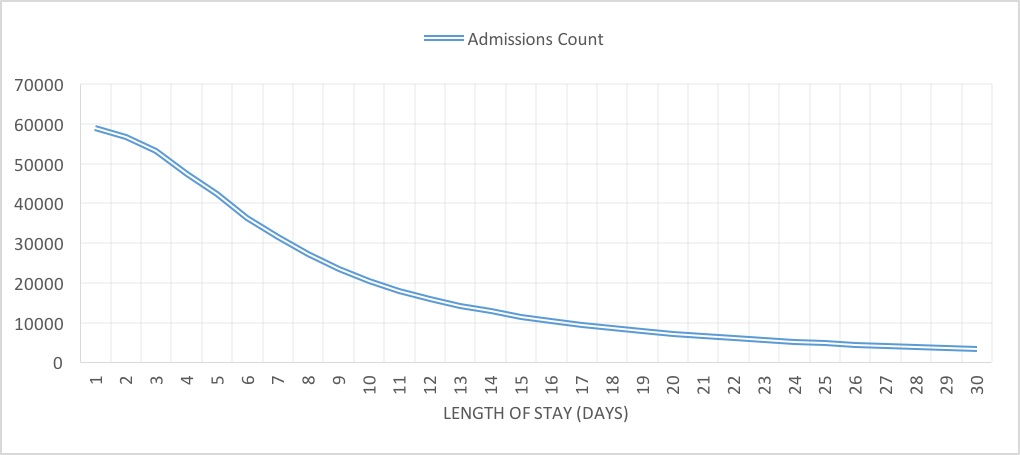
\includegraphics[width=8cm]{admission_count}
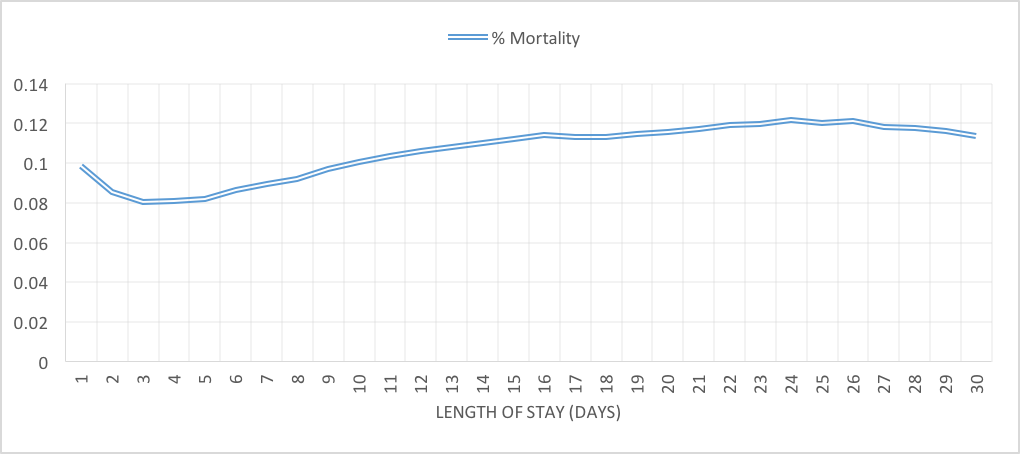
\includegraphics[width=8cm]{percent_mortality}
\caption{Top:  Total number of remaining admissions as a function of number of days in the hospital.  Bottom:  Percent of remaining admissions that result to an in-hospital mortality event as a function of the number of days in the hospital.}
\end{figure}

\subsection{Experimental Results}

The retrospective analysis of our process was done by rerunning the entire model building process on a 10-Fold cross validation where 70\% of the data was used to rebuild the model and than score the AUC on the remaining 30\%.   The AUCs ranged between 0.869 and 0.909 with an average of 0.878.

The time-varying evaluation of the model is shown in Figure 2.   The bottom (blue) line is just using the admission time as a baseline.  This prediction is made from the first 24 hours of data, and is not updated at any point after this initial prediction.  The fact that the model’s ability discriminates the severity of patients as their time in the hospital increase is expected.  The middle (orange) curve is a logistic model built only on the time varying topics.  This model is much better than the admission-based model on discriminating the severity of patients.  It is unexpected that the model’s ability to discriminate severity after 5 days degrades.   More clinical notes add predictive power in the beginning, but do not continue over time.   This suggests that a rolling window of notes might be better than a pure combination of all clinical notes.   The top (gray) line is the final time-varying model that uses admission-based features as well as time varying topics.  At a high level, the results of this analysis match the results from Ghassemi et. al. for the combined model predicting in-hospital model events.

\begin{figure}[ht]
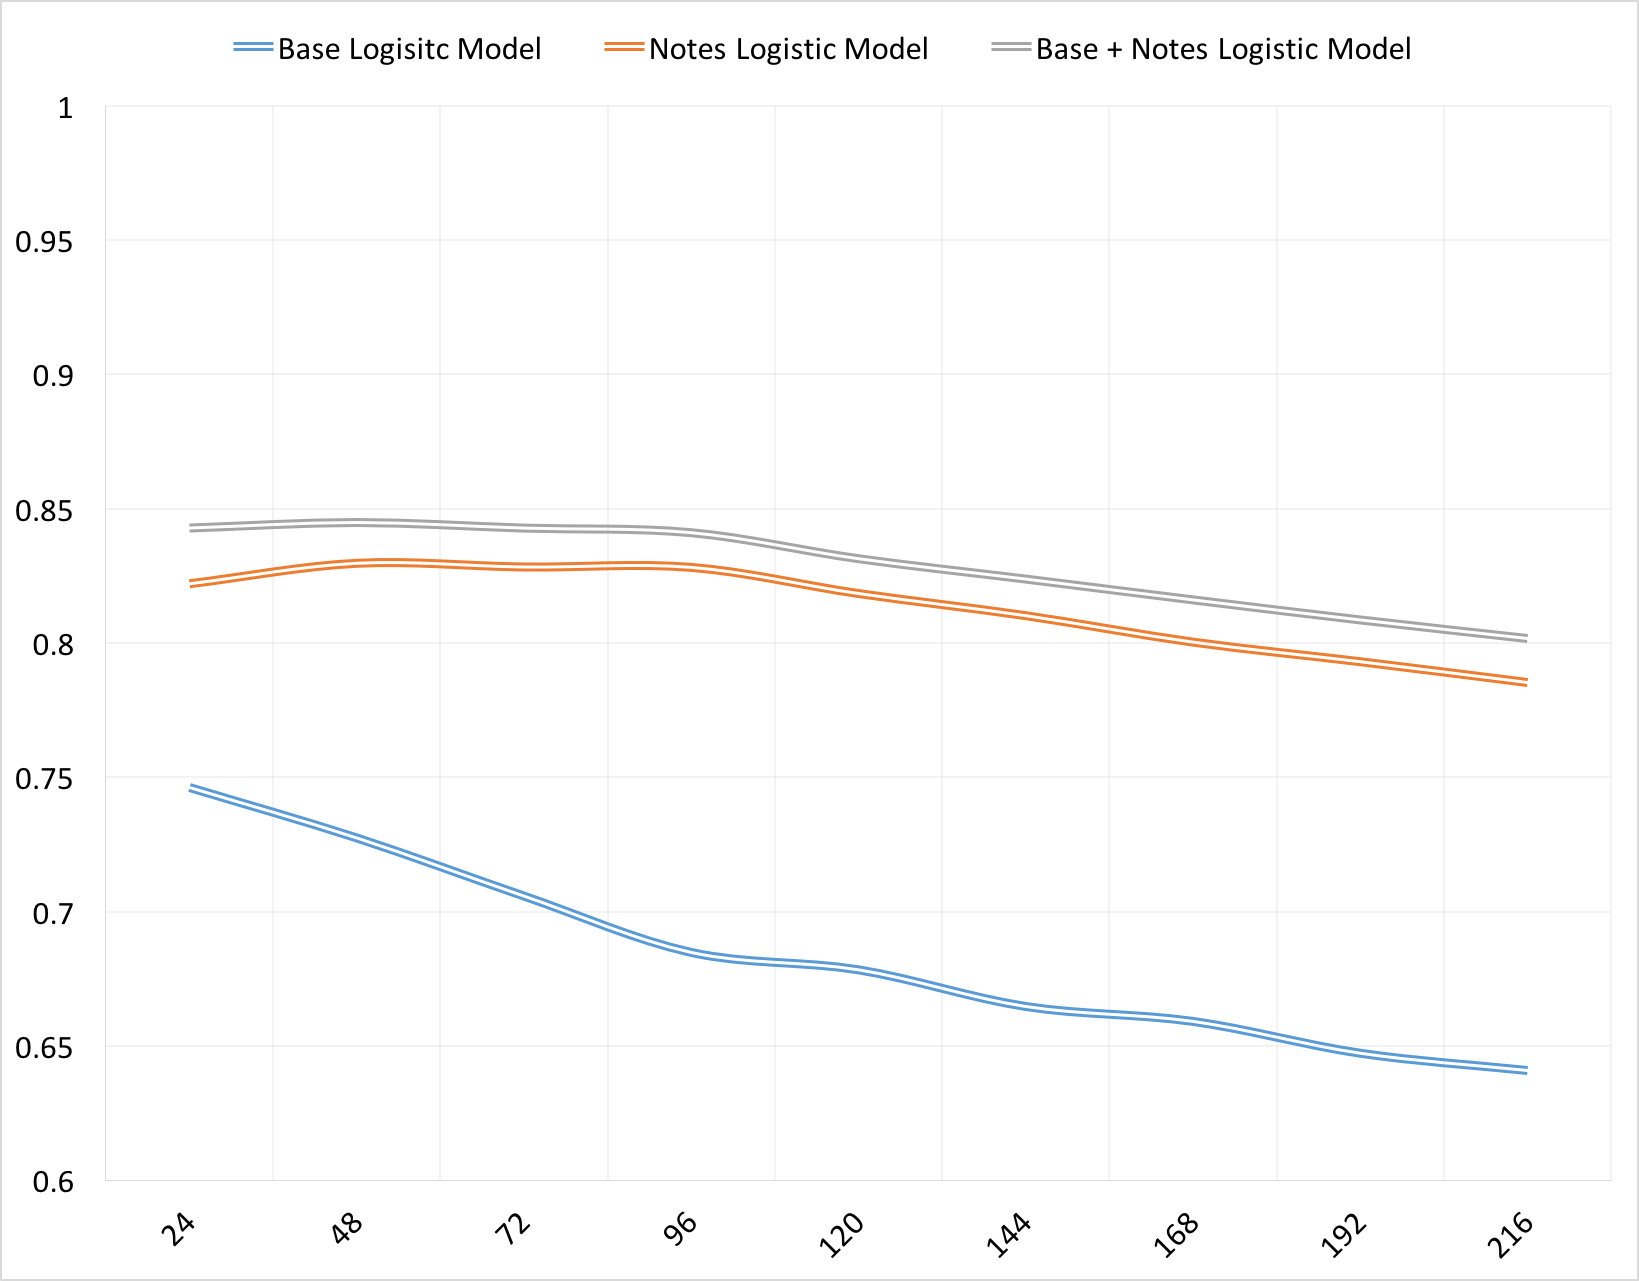
\includegraphics[width=8cm]{auc}
\caption{Graph of AUC of model predictions on test data for time-varying features.   The bottom (blue) line is the baseline admission model. The middle (orange) line is the performance of a model based only on topics.  The top (gray) line is the performance of the final model using both admission data and note topics.}
\end{figure}


\section{Conclusions}

This work was motivated by Ghassemi et. al.’s  discovery that there is rich and useful information in hospital notes that inform a given patient's severity and that time-varying models could potentially be useful in a hospital context.  Real-time models require streaming context and a large amount of data, so reproducing their work in Scala with Apache Spark is a step towards scalable real-time medical predictions as well as a validation of the process of using clinical notes is informative in prediction patient outcomes.

Despite the increase rate of in-hospital mortality with longer hospital states, the MIMIC III dataset highlights that the window of time with the most mortalities is the first 24 hours.  This windows makes up 16.7\% of all mortalities in the dataset.  The model in this paper is not capable of scoring these patients before they have died.

Another limitation of the current work can be seen in examining topic 5 of appendix A.  It shows an exceptionally high odds-ratio for mortality in the model.  The top 20 words for this topic is associated with automobile accidents.  Despite being able to describe the severity of this event, and the LDA creating a topic for it, a model for the severity of this condition is likely not adding information that the medical practitioner in the hospital do not already have.

Topics 10 and 18 both have the words pt and goal.  Each of these topics topics have odds ratios less than 1, and the words in these topics appear to be associated with recovery.  The model describes them as associated with lower risk of mortality.   The issue with this aspect of the process and model is that the information is in the system after a doctor has applied judgment to order physical therapy and a physical therapist has engaged the patient.   In these cases, the model is reflecting back practitioners' judgment instead of augmenting it.  

In both of the above examples, the model is accurately capturing in-hospital mortality risk, but in situations that are not possible to predict.  The value-add for severity scores are in situations where the immediate risk is not obvious to an experienced medical practitioner.  It seems that models built on clinical notes are capable of capturing and describing a patient's states and risks of in-hospital mortality.  It also appears that some of the clinical notes capture the physician's judgment about the severity of the patient's condition, and the prediction system reflects this back after the notes have been processed.

There is more work to be done to determine the optimal type and range of features to be included in streaming medical reporting and prediction systems.   The information and prediction should be informative and predictive to be both practical and useful.  Clinical notes have been confirmed to be informative in our work.  The subtlety in how they are used to generate predictive features still needs to be discovered.    


% use section* for acknowledgment
% \section*{Acknowledgment}
% TBD - Bryan's Super Awesome Ackowledgement Secion of Gracious Professionalism

%\bibliography{cse8803project}
%\bibliographystyle{abbrv}
\begin{thebibliography}{1}

\bibitem{ghassemi_unfolding_2014}
M.~Ghassemi, T.~Naumann, F.~Doshi-Velez, N.~Brimmer, R.~Joshi, A.~Rumshisky,
  and P.~Szolovits.
\newblock Unfolding {Physiological} {State}: {Mortality} {Modeling} in
  {Intensive} {Care} {Units}.
\newblock In {\em Proceedings of the 20th {ACM} {SIGKDD} {International}
  {Conference} on {Knowledge} {Discovery} and {Data} {Mining}}, {KDD} '14,
  pages 75--84, New York, NY, USA, 2014. ACM.

\bibitem{mozomi_2015}
Nozomi Nori , Hisashi Kashima , Kazuto Yamashita , Hiroshi Ikai , Yuichi Imanaka, 
\newblock Simultaneous Modeling of Multiple Diseases for Mortality Prediction in Acute Hospital Care, 
\newblock In {\em Proceedings of the 21th {ACM} {SIGKDD} {International} {Conference} on {Knowledge} {Discovery} 
and {Data} {Mining}}, August 10-13, 2015, Sydney, NSW, Australia

\bibitem{ghassemi_2015}
Marzyeh Ghassemi , Marco A. F. Pimentel , Tristan Naumann , Thomas Brennan , David A. Clifton , Peter Szolovits , Mengling Feng, 
\newblock A multivariate time-series modeling approach to severity of illness assessment and forecasting in ICU with sparse, heterogeneous clinical data, 
\newblock In {\em {Proceedings} of the {Twenty-Ninth} {AAAI} {Conference} on {Artificial} {Intelligence}}, p.446-453, January 25-30, 2015, Austin, Texas

\bibitem{caballero_2015}
Karla L. Caballero, Ram Akella, 
\newblock Dynamically Modeling Patient's Health State from Electronic Medical Records: A Time Series Approach, 
\newblock In {\em {Proceedings} of the {21th} {ACM} {SIGKDD} {International} {Conference} on {Knowledge} {Discovery} 
and {Data} {Mining}}, August 10-13, 2015, Sydney, NSW, Australia



\bibitem{saeed_multiparameter_2011}
M.~Saeed, M.~Villarroel, A.~T. Reisner, G.~Clifford, L.-W. Lehman, G.~Moody,
  T.~Heldt, T.~H. Kyaw, B.~Moody, and R.~G. Mark.
\newblock Multiparameter {Intelligent} {Monitoring} in {Intensive} {Care} {II}:
  a public-access intensive care unit database.
\newblock {\em Critical Care Medicine}, 39(5):952--960, May 2011.


\end{thebibliography}

\onecolumn
\begin{appendices}
\section{Top 20 Words and Odd-Ratio for each topic}
\begin{center}
    \begin{longtable}{| p{.05\textwidth} | p{.05\textwidth} | p{.8\textwidth}|}
    \hline
    Topic & Odds Ratio &  Top 20 Words \\ \hline
  1 & 31.9 & fx, fracture, ortho, rib, hip, action, assessment, trauma, fractures, orif, femur, fusion, pain, response, injuries, medications, dilaudid, knee, brace, laceration \\ \hline
  2 & 5.2 & infant, nicu, sepsis, baby, maternal, cbc, gbs, parents, nursery, term, newborn, murmur, intrapartum, born, normal, nbn, pregnancy, warmer, delivery, fetal \\ \hline
  3 & 2.3 & dementia, mental, history, assessed, javascript, altered, icu, popup, meq, pulse, webtag, action, fever, medications, pneumonia, patient, assessment, myeloma, mri, alzheimer \\ \hline
  4 & 0.56 & lap, tpn, colectomy, ileostomy, date, assessment, action, jp, ex, tube, resection, dilaudid, abdominal, acute, ostomy, comments, flush, fistula, drain, abscess \\ \hline
  5 & 111241 & tonic, mandibular, clonic, pedestrian, flolan, struck, mandible, obstipation, frx, fos, fx, seizure, mirapex, pubic, pvi, epilepsy, rami, omfs, car, tendon \\ \hline
  6 & 1.7 & bleed, gib, action, assessed, assessment, meq, brbpr, medications, comments, icu, history, ul, pulse, abdominal, balance, bleeding, colonoscopy, response, egd, sbo \\ \hline
  7 & 0.02 & infant, caffeine, pn, cares, il, lastname, feeds, cbg, isolette, fio, retractions, wt, baby, mom, spells, murmur, settings, servo, spits, diuril \\ \hline
  8 & 8.1e-4 & crrt, hd, cvvh, dialysis, sle, cryptogenic, renal, wound, cvvhd, cirrhosis, lupus, transplant, sirs, cvvhdf, anuric, vac, liver, hemodialysis, paracentesis, crf \\ \hline
  9 & 0.58 & cmh, trach, comments, ards, failure, assessed, assessment, ventilation, tube, peg, tracheostomy, meq, ul, respiratory, airway, pna, action, pneumonia, medications, lung \\ \hline
  10 & 0.12 & trach, vent, icp, secretions, collar, drain, propofol, coarse, tf, sicu, pt, peg, remains, tragus, eyes, suctioned, goal, psv, intubated, mannitol \\ \hline
  11 & 1.4 & evd, hemorrhage, icp, brain, headache, nicardipine, aneurysm, date, mannitol, stroke, mri, cerebral, mass, nimodipine, assessment, ich, vasospasm, checks, sah, cerebellar \\ \hline
  12 & 0.9 & transplant, liver, crrt, renal, kidney, failure, cirrhosis, cvvh, micafungin, olt, hepatic, tacrolimus, splenectomy, action, assessment, esld, hepatorenal, arf, dobhoff, acute \\ \hline
  13 & 24.4 & neo, iabp, ci, csru, wires, svo, gtt, ntg, lasix, percocet, pacer, endo, milrinone, ct, wean, insulin, drainage, epi, propofol, cabg \\ \hline
  14 & 58.4 & stemi, nstemi, rca, lad, ccu, cath, plavix, action, cad, lcx, infarction, myocardial, ami, stent, carotid, cp, coronary, pci, asa, artery \\ \hline
  15 & 1.1 & pt, ccu, micu, bipap, sob, wife, confused, cooperative, npn, cath, ew, denies, bed, gu, gtt, nc, lasix, sitter, gi, commode \\ \hline
  16 & 550.6 & etoh, valium, ciwa, withdrawal, pancreatitis, abuse, ercp, hiv, alcohol, cholangitis, lipase, action, thiamine, dts, assessment, assessed, tremens, diazepam, delirium, seizures \\ \hline
  17 & 5.8e-3 & infant, cares, feeds, mom, active, aquaphor, cc, benign, wt, neonatology, cont, tf, spits, caffeine, ccu, milrinone, pe, voiding, day, remains \\ \hline
  18 & 0.17 & trach, vent, secretions, peep, coarse, pt, suctioned, ps, psv, tube, remains, gtt, sputum, settings, abg, lasix, white, tf, mdi, goal \\ \hline
  19 & 244.0 & egd, endoscopy, varices, nephrostomy, octreotide, melena, esophageal, bleed, charcot, bleeding, banding, scope, esophagus, cbi, variceal, ent, hematemesis, pheresis, angioedema, protonix \\ \hline
  20 & 13.6 & serratia, citrobacter, polymyalgia, infant, duodenal, iabp, enteroscopy, rheumatica, osh, action, jejunal, assessment, iodine, cares, feeds, assessed, vioxx, comments, mom, eclampsia \\ \hline
  21 & 1.3e-6 & arrest, pea, versed, fentanyl, vent, peep, intubated, eeg, anoxic, sedation, mcg, sedated, unresponsive, cooling, ett, gtt, secretions, ac, propofol, trach \\ \hline
  22 & 5.2 & svg, pod, assessment, bypass, action, cabg, graft, cmh, avr, pedis, coronary, dorsalis, meq, cvicu, aspirin, temporary, medications, artery, response, tibial \\ \hline
  23 & 0.79 & pancreatitis, ercp, pancreatic, pancreas, pseudocyst, necrotizing, mrcp, maze, cbd, knee, duct, peripancreatic, ligation, cholestasis, biliary, drain, dilaudid, hida, gallstones, necrosis \\ \hline
  24 & 9.7e-3 & failure, action, cmh, assessment, assessed, acute, ards, renal, arf, shock, levophed, comments, response, meq, hypotension, ul, pressors, meropenem, pulse, sepsis \\ \hline
  25 & 0.08 & sdh, sah, dilantin, seizure, hemorrhage, subdural, assessment, trauma, temporal, action, keppra, comments, cmh, famotidine, fall, epilepticus, subarachnoid, trach, eeg, fracture \\ \hline
  26 & 0.01 & lactulose, cirrhosis, liver, encephalopathy, hepatic, ascites, paracentesis, assessed, tips, portal, action, rifaximin, meq, pulse, comments, medications, albumin, hcv, assessment, failure \\ \hline
  27 & 3.9 & copd, assessed, history, meq, bipap, action, icu, medications, comments, assessment, pulse, exacerbation, balance, acute, patient, unknown, ed, overdose, nebs, schizophrenia \\ \hline
  28 & 3.0 & hd, esrd, dialysis, renal, stage, pd, assessed, chronic, action, kidney, assessment, abscess, failure, crf, meq, bacteremia, pulse, mssa, urosepsis, comments \\ \hline
  29 & 1.0 & icd, ep, paced, ablation, vt, ccu, pacer, av, amiodarone, aicd, firing, pacemaker, pacing, lidocaine, block, chb, ppm, dobutamine, milrinone, lido \\ \hline
  30 & 0.09 & bmt, gvhd, dka, sct, bactrim, acyclovir, bal, gap, viremia, voriconazole, ards, smx, insulin, tmp, cmv, ketoacidosis, gastroparesis, pcp, vre, viral \\ \hline
  31 & 9.7e-3 & aortic, milrinone, valve, endocarditis, nafcillin, mssa, action, bacteremia, mitral, lasix, mvr, assessment, chf, avr, tee, failure, valvuloplasty, ef, meq, septic \\ \hline
  32 & 0.02 & thalamic, infant, transplant, action, feeds, liver, assessment, caffeine, cares, esld, landing, cirrhosis, serratia, spells, spits, brainstem, dobhoff, comments, active, mom \\ \hline
  33 & 14.4 & infant, cares, feeds, mom, spells, spits, wt, isolette, crib, voiding, active, dev, caffeine, retractions, swaddled, neonatology, pacifier, stooling, fen, pg \\ \hline
  34 & 1.6e-2 & pericardial, effusion, cancer, metastatic, lymphoma, chemo, onc, malignant, chemotherapy, tamponade, cell, pleural, oncology, mets, tumor, neoplasm, drain, mass, xrt, follicular \\ \hline
  35 & 0.4 & fibrillation, atrial, chf, afib, coumadin, rvr, lasix, action, assessed, heparin, failure, heart, chronic, diastolic, history, assessment, diltiazem, cad, response, acute \\ \hline
    \end{longtable}
\end{center}

\end{appendices}

\end{document}
